\section{Incorporation of Dynamic Tubes for Constraint Satisfaction}
\label{sec:dynamic-tube}
\begin{figure*}[htb]
    \centering
    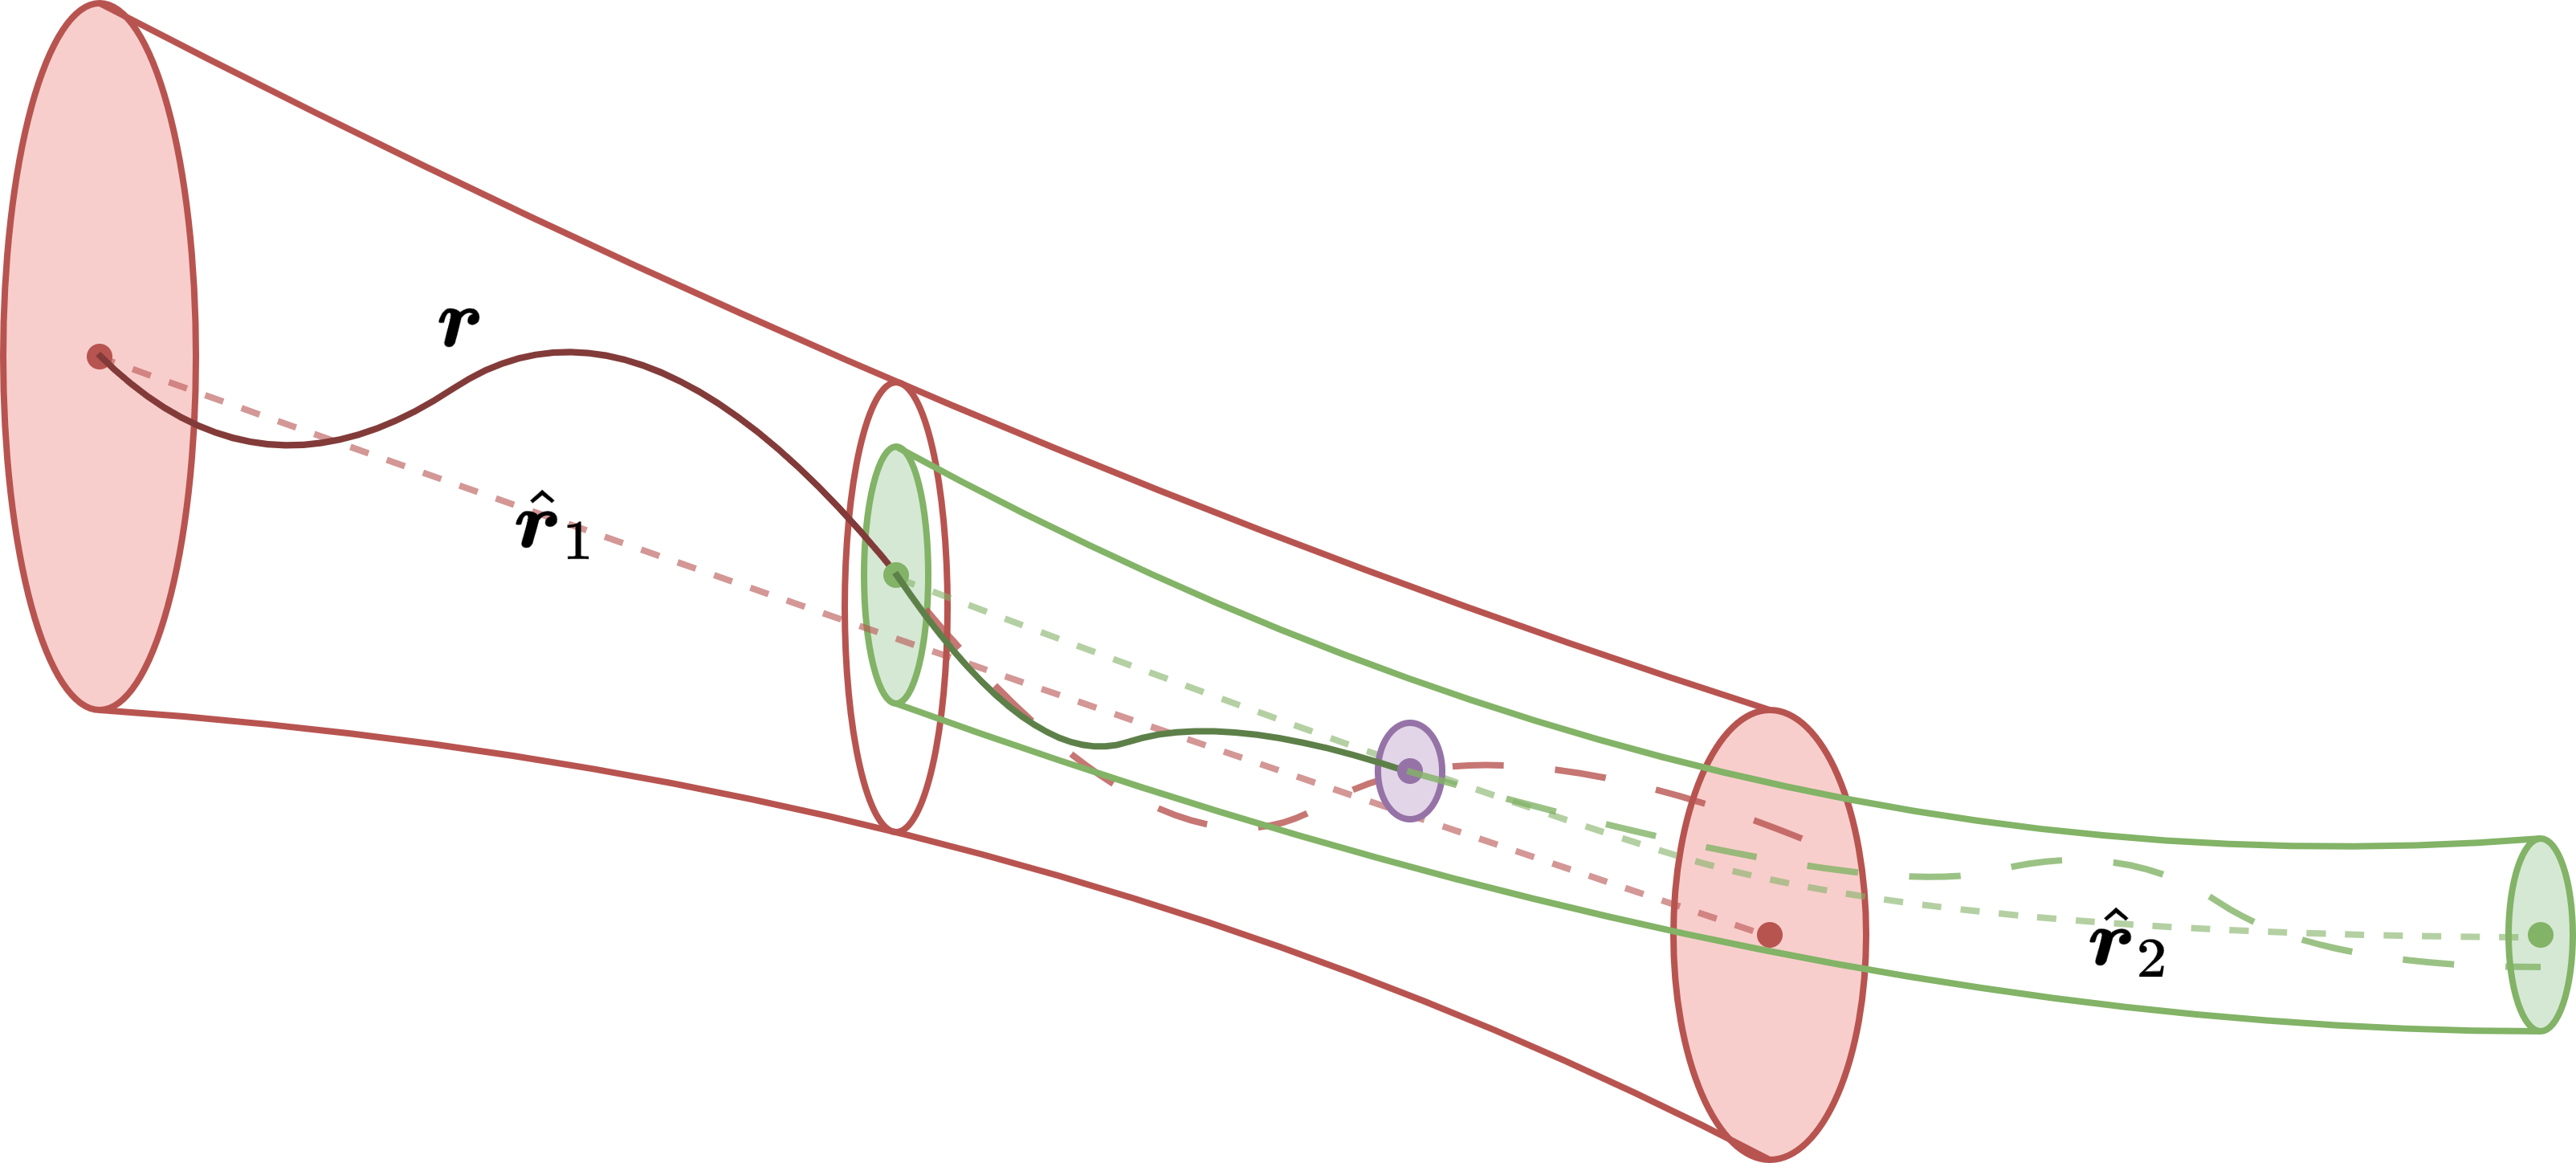
\includegraphics[width = 0.9\textwidth]{assets/adtmpc.png}
    \caption{\textbf{Adaptive Tube Model Predictive Control}: The tubes represent the permissible region for the actual trajectory of the chaser. The dotted lines represent the nominal states and the dashed lines represent the actual states. Due to the receding horizon nature of the problem, the spacecraft plans a new trajectory before the final state is reached.}
    \label{fig:adtmpc}
\end{figure*}
Following the determination of the docking point of the chaser, the chaser plans a trajectory from the current position to the calculated goal position on the target.
By the completion of rendezvous, the chaser has a significantly accurate estimate for uncertain parameters such as eccentricity and drag coefficients and it is capable of planning a trajectory from a start position to a docking point on the target.
However, the high degree of proximity and physical contact required for docking increases the likelihood of a chaser-target collision.
This is theoretically avoided using the time-varying docking constraint explained in Section \ref{sec:time-varying-collision-constraints}.
However, the inaccuracy in estimated parameters may lead to a violation of this constraint.
In order to avoid such constraint violations, we use dynamic robust control-invariant (RCI) tubes as proposed in \cite{brett2019dynamic} to constrain the possible error in the chaser state, hence using adaptive dynamic tube MPC (ADTMPC) for chaser trajectory planning.
As a result, the nominal trajectory planning problem for docking can be formulated as the following optimization problem:
\begin{align}
    \min_{\hat{\boldsymbol{r}}, \hat{\boldsymbol{u}}, \hat{\boldsymbol{v}}}\ &J(\hat{\boldsymbol{r}}(\theta),\hat{\boldsymbol{u}}(\theta))=\int_{\theta_0}^{\theta_f}\left(\hat{\boldsymbol{u}}^T(\theta)R\hat{\boldsymbol{u}}(\theta)\right)d\theta
\end{align}
\begin{subequations}
\begin{align}
    \textrm{s.t. } & \hat{\boldsymbol{r}}'(\theta)=A(\theta)\hat{\boldsymbol{r}}(\theta)+B(\theta)\hat{\boldsymbol{u}}(\theta)+\hat{\boldsymbol{d}}(\theta), \ \ \hat{\boldsymbol{u}}\in\hat{\mathbb{U}},\\
    & \hat{\boldsymbol{r}}(\theta_0)=\boldsymbol{r}(\theta_0)=\boldsymbol{r}_0, \quad\zeta(\hat{\boldsymbol{r}}(\theta_f))=0,\quad{\mathcal{C}}>0,\\
    & \hat{\boldsymbol{\alpha}}'(\theta)=\hat{\boldsymbol{v}}(\theta), \ \ \hat{\boldsymbol{\alpha}}(\theta_0)=\boldsymbol{\alpha}_0, \ \ \hat{\boldsymbol{\alpha}}(\theta)\in{\mathbb{A}}, \ \ \hat{\boldsymbol{v}}(\theta)\in{\mathbb{V}},\\
    & \boldsymbol{\phi}'(\theta)=-[\hat{\boldsymbol{\alpha}}(\theta)][\boldsymbol{\phi}(\theta)]+\boldsymbol{\Delta}(\hat{\boldsymbol{r}}(\theta))+\boldsymbol{D}+\boldsymbol{\eta},\ \ \boldsymbol{\phi}(\theta_0)=\boldsymbol{\phi}_0,\\
    & \boldsymbol{\Omega}'(\theta)=A_\lambda\boldsymbol{\Omega}(\theta)+B_\lambda\boldsymbol{\phi}(\theta),\quad\boldsymbol{\Omega}(\theta_0)=|\Tilde{\boldsymbol{r}}_0|
    \label{eqn:docking-problem}
\end{align}
\end{subequations}
where $A_\lambda=\text{diag}(\boldsymbol{\lambda})=\text{diag}(\{\lambda_i,i=1,2,3\})$ and $B_\lambda=I_{3}$ are predefined, and $[\boldsymbol{v}]=\text{diag}(\boldsymbol{v})$ for a vector $\boldsymbol{v}$.
Here, $\phi(\theta)$ represents the boundary layer of the tube and $\Omega(\theta)$ represents the tube geometry.
\subsection{Ancillary Controller and the Actual Control Input}
In light of the proposed uncertainties and the dynamic tube mechanism to deal with them, we implement control input modification as proposed originally in the DTMPC algorithm \cite{brett2019dynamic} since it provides recursive feasibility to the MPC problem.
The actual control input $\boldsymbol{u}$ can be written as the sum of the nominal input $\hat{\boldsymbol{u}}$ and an ancillary controller $\Tilde{\boldsymbol{u}}$ based on boundary-layer sliding control (BLSC):
\begin{alignat}{2}
    \boldsymbol{u}&=\hat{\boldsymbol{u}}+\Tilde{\boldsymbol{u}}\\
    \Tilde{\boldsymbol{u}}&=B(\boldsymbol{r})^{-1}\left(A^V\Tilde{\boldsymbol{r}}-A_\lambda\Tilde{\boldsymbol{r}}^V-[K(\boldsymbol{r})]\left[\text{sat}\left(\frac{\boldsymbol{s}}{\boldsymbol{\phi}}\right)\right]\right)
\end{alignat}
where the sliding variable $\boldsymbol{s}$ is defined as:
\begin{alignat}{2}
    \boldsymbol{s}=\Tilde{r}^V+A_\lambda\Tilde{r}^P,
\end{alignat}    
and $K(\boldsymbol{r})$ can be calculated as:
\begin{alignat}{2}
    \boldsymbol{\phi}'&=-[\boldsymbol{\alpha}][\boldsymbol{\phi}]+\boldsymbol{\Delta}(\boldsymbol{r}(\theta))+\boldsymbol{D}+\boldsymbol{\eta}\\
    K(\boldsymbol{r})&=\boldsymbol{\Delta}(\boldsymbol{r}(\theta))+\boldsymbol{D}+\boldsymbol{\eta}-\phi'\\
    &=(\boldsymbol{\Delta}(\boldsymbol{r}(\theta))-\boldsymbol{\Delta}(\hat{\boldsymbol{r}}(\theta)))+[\boldsymbol{\alpha}][\boldsymbol{\phi}]\\
    &=\boldsymbol{\Delta}(\Tilde{\boldsymbol{r}}(\theta))+[\boldsymbol{\alpha}][\boldsymbol{\phi}].\label{eqn:K(r)}
\end{alignat}
Here, $\boldsymbol{\Delta}(\boldsymbol{r}(\theta))$ is the maximum bound on the dynamics $\boldsymbol{f}=\hat{\boldsymbol{f}}+\Tilde{\boldsymbol{f}}$ where $\hat{\boldsymbol{f}}$ is the nominal dynamics and $\Tilde{\boldsymbol{f}}$ is the bounded model error such that $|\Tilde{\boldsymbol{f}}|\leq\boldsymbol{\Delta}(\boldsymbol{r}(\theta))$.
Also, $\boldsymbol{D}$ is the maximum bound on the disturbance $\boldsymbol{d}(\theta)$ in the dynamics such that $\boldsymbol{d}(\theta)\leq\boldsymbol{D}$, and $\boldsymbol{\eta}$ is a predefined quantity.
\subsection{Shrinking of State and Input Bounds}
\label{sec:bound-shrinking}
State and input constraints need to be modified due to the non-zero tracking error $\Tilde{\boldsymbol{r}}(\theta)$. The state and input bounds defined in Section \ref{sec:state-input-bounds} must be modified to account for the non-zero tracking error and control input error. We incorporate the tightening equations proposed in \cite{brett2019dynamic} as follows:
\begin{align}
    ||P_{\hat{\boldsymbol{r}}}\boldsymbol{r}(\theta)+q_{\hat{\boldsymbol{r}}}||&\leq C_{\hat{\boldsymbol{r}}}-||P_{\hat{\boldsymbol{r}}}\Tilde{\boldsymbol{r}}(\theta)||\\
    ||P_{\hat{\boldsymbol{u}}}\overline{B}^{-1}\hat{\boldsymbol{u}}(\theta)+q_{\hat{\boldsymbol{u}}}||&\leq C_{\hat{\boldsymbol{u}}}-||P_{\hat{\boldsymbol{u}}}\overline{B}^{-1}\Tilde{\boldsymbol{u}}_{fb}||
\end{align}
In our problem, we may write this (for $i=1,2,3$) as:
% \begin{align}
%     ||\boldsymbol{r}^P(t)||_\infty&<    \infty\quad\text{(no bound)}\\
%     ||\boldsymbol{r}^V(t)||_\infty&\leq C_{\boldsymbol{r}^V}-||\boldsymbol{r}^V(t)||_\infty\\
%     ||\boldsymbol{u}  (t)||_\infty&\leq C_{\boldsymbol{u}}
% \end{align}
\begin{align}
    |r_i^P(\theta)|&<    \infty\quad\text{(no bound)},\\
    |r_i^V(\theta)|&\leq C_{r^V}-|\Tilde{r}^V|,\\
    |u_i  (\theta)|&\leq C_{u}-|\Tilde{u}_{fb,i}|,
\end{align}
such that
\begin{subequations}\label{fourth:main}
\begin{alignat}{2}
    \Tilde{\boldsymbol{u}}_{fb}&=\left|\overline{F}+A_{\lambda}\Tilde{\boldsymbol{r}}\right.&&\left.+\overline{K}\right|\tag{\ref{fourth:main}}\\
    \overline{\boldsymbol{F}}&=A^V\overline{\boldsymbol{r}},&&\underline{\boldsymbol{F}}=A^V\underline{\boldsymbol{r}}\\
    \overline{\boldsymbol{K}}&=K\left(\overline{\boldsymbol{r}}\right),&&\underline{\boldsymbol{K}}=K\left(\underline{\boldsymbol{r}}\right)\\
    \overline{\boldsymbol{r}}&=\hat{\boldsymbol{r}}+|\Tilde{\boldsymbol{r}}|,&&\underline{\boldsymbol{r}}=\hat{\boldsymbol{r}}-|\Tilde{\boldsymbol{r}}|
\end{alignat}
\end{subequations}
where $K(\cdot)$ is defined in Equation \ref{eqn:K(r)}.
\subsection{Expansion of (Concave) State Constraints}
We realize that, although the inputs are bound in a convex space, the state space is non-convex either due to the radial-limit constraint (Equation \ref{eqn:radial-limit-constraint}) during rendezvous or due to the target-limit constraint (Section \ref{sec:time-varying-collision-constraints}) during docking.
These constraints need to be expanded resembling how the convex bounds are shrunk in Section \ref{sec:bound-shrinking}.
As a result, the radial-limit constraint can now be rewritten as:
\begin{align}
    ||\boldsymbol{r}^P(\theta_f)||>r_{\text{Target}}+||\Tilde{\boldsymbol{r}}^P|| \label{eqn:expanded-radial-limit-constraint}
\end{align}
Now, the target-limit constraint must be expanded such that the dynamic RCI tube can at most touch the target.
However, since distances are invariant to rotations, the expansion of the constraint is not affected by the rotation of the position of the chaser with respect to the target.
As a result, the target-limit constraint in Equation \ref{eqn:or-function} can be rewritten as follows:
\begin{subequations}\label{fifth:main}
\begin{align}
    {\mathcal{C}}_D&={\mathcal{C}}_{D1}\cup{\mathcal{C}}_{D2}\label{eqn:expanded-target-limit-constraint}\tag{\ref{fifth:main}}\\
    {\mathcal{C}}_{D1}&=\{\boldsymbol{r}(\theta):f_{D1}\geq0\}\\
    {\mathcal{C}}_{D2}&=\{\boldsymbol{r}(\theta):f_{D2}\geq0\}
\end{align}
\end{subequations}
where
\begin{subequations}
\begin{align}
    f_{D1}&=x_{\mathcal{R}}(\theta)^2 + y_{\mathcal{R}}(\theta)^2 - (r_T+||\Tilde{\boldsymbol{r}}^P||)^2\\
    f_{D2}&=||z_{\mathcal{R}}(\theta)|| - (l_T+||\Tilde{\boldsymbol{r}}^P||)
\end{align}
\end{subequations}
We realize that this can be slightly conservative on the edges of the target.
This can be rectified by adding a third constraint while ignoring the existing two constraints at the edge to provide a rounded cylinder constraint.
We do not address the equations for the same here but encourage the reader to do the same.
Moreover, it can be made less conservative by constraining each dimension separately, giving:
\begin{subequations}
\begin{align}
    f_{D1}&=x_{\mathcal{R}}(\theta)^2 + y_{\mathcal{R}}(\theta)^2 - (r_T+||\begin{bmatrix}
        \Tilde{x}_{\mathcal{R}}&\Tilde{y}_{\mathcal{R}}
    \end{bmatrix}||)^2\\
    f_{D2}&=||z_{\mathcal{R}}(\theta)|| - (l_T+||\Tilde{z}_{\mathcal{R}}||)
\end{align}
\end{subequations}
where, for $r_i\in[x,y,z]$,
\begin{align}
    \Tilde{r}_{i, {\mathcal{R}}}=r_{i, {\mathcal{R}}}(\theta)-\hat{r}_{i, {\mathcal{R}}}(\theta)
\end{align}